\begin{question}{11}
Describe a Turing machine that decides whether all symbols in an input string are distinct. Assume the input alphabet is finite. Explain why the machine always halts.
\end{question}
\begin{soln}
\textbf{Idea.} Take the symbols one at a time as a ``pivot'' and check that the pivot does not occur again to its right. Since $\Sigma$ is finite, the machine can \emph{remember the pivot symbol in its state} (one copy of the scanning states for each $\sigma\in\Sigma$).

$M=$ ``On input $w$:
\begin{enumerate}
\item Mark the left end (replace the first symbol $a$ by a special version $\hat a$, which still counts as the symbol $a$), so the machine can find it again.
\item Find the leftmost unmarked symbol $\sigma$. If there is none, \emph{accept}. Otherwise mark it as $\dot\sigma$ and remember $\sigma$ in the state.
\item Scan right to the end of the input. If an unmarked $\sigma$ is seen, \emph{reject}.
\item Return to the left end and go to stage 2.''
\end{enumerate}

\textbf{Correctness.} If $w_i=w_j$ with $i<j$, then when $w_i$ is the pivot, stage 3 sees $w_j$ and rejects. If all symbols are distinct, no scan ever rejects, and after $|w|$ rounds everything is marked: accept.

\textbf{Halting.} Every round marks one more cell, so there are at most $|w|+1$ rounds, and each round is one sweep right and one sweep back over $|w|$ cells (at most $O(|w|^2)$ steps in total). Finiteness of $\Sigma$ is what makes ``remember $\sigma$'' possible with finitely many states.

(Shortcut: if $|w|>|\Sigma|$ the answer is ``no'' by the pigeonhole principle, but the machine above does not need this.)
\end{soln}

\begin{question}{12}
Explain the difference between a Turing machine that recognizes a language and one that decides a language.
\end{question}
\begin{soln}
On an input, a TM can \emph{accept}, \emph{reject}, or \emph{loop} (run forever).
\begin{itemize}
\item $M$ \textbf{recognizes} $L$ if $L=L(M)=\{w\mid M\text{ accepts }w\}$. On $w\notin L$ it may reject \emph{or loop}.
\item $M$ \textbf{decides} $L$ if it recognizes $L$ \emph{and halts on every input}: it accepts every $w\in L$ and rejects every $w\notin L$.
\end{itemize}
So a recognizer gives a guaranteed ``yes'' answer, but for a ``no'' you may wait forever without learning anything. A decider always answers.

Every decider is a recognizer, so decidable $\subseteq$ Turing-recognizable. The inclusion is strict: $\Atm=\{\enc{M,w}\mid M \text{ accepts } w\}$ is recognized by the universal TM (simulate $M$ on $w$), which loops when $M$ loops, and no TM decides $\Atm$ (Sipser Thm 4.11).
A useful fact: $L$ is decidable $\iff$ both $L$ and $\comp L$ are Turing-recognizable (Thm 4.22).
\end{soln}

\begin{question}{13}
Explain why allowing a Turing machine's head to stay in place during a transition does not increase its computational power. Describe how such a transition can be simulated by a standard Turing machine.
\end{question}
\begin{soln}
A ``stay'' model has $\delta:Q\times\Gamma\to Q\times\Gamma\times\{L,R,S\}$.

\textbf{Simulation.} Replace each stay move $\delta(q,a)=(r,b,S)$ by two ordinary moves through a new state $p$:
\[
\delta(q,a)=(p,\,b,\,R),\qquad \delta(p,c)=(r,\,c,\,L)\quad\text{for every }c\in\Gamma .
\]
That is: write $b$ and step right, then step back left without changing anything. The result is the same configuration (cell is $b$, head on the same cell, state $r$), reached in two steps instead of one. All $L/R$ moves are copied unchanged.

\emph{Why right-then-left?} The tape has a left end, and a left move from the leftmost cell does not move the head. A right move always moves, so ``right then left'' always returns to the same cell.

\textbf{No extra power.} Each step of the stay-machine becomes one or two steps of the standard machine, so both accept, reject and loop on exactly the same inputs. Conversely, a standard TM is a stay-TM that never uses $S$. Hence both models recognize (and decide) the same languages.
\end{soln}

\begin{question}{14}
Show that every multitape Turing machine can be simulated by a single-tape Turing machine. Explain the representation of the multiple tapes and head positions on the single tape.
\end{question}
\begin{soln}
(Sipser Thm 3.13.) Let $M$ have $k$ tapes. We build a single-tape TM $S$.

\textbf{Representation.} Write the contents of the $k$ tapes one after another, separated by $\#$. Mark each head position by putting a \emph{dot} on the symbol under that head; so for every $a\in\Gamma$ the tape alphabet of $S$ contains both $a$ and $\dot a$, plus $\#$:
\[
\#\;\underbrace{\cdots\dot a\cdots}_{\text{tape 1}}\;\#\;\underbrace{\cdots\dot b\cdots}_{\text{tape 2}}\;\#\;\cdots\;\#\;\underbrace{\cdots\dot c\cdots}_{\text{tape }k}\;\#
\]

\begin{center}
\begin{tikzpicture}[cell/.style={draw,minimum width=0.62cm,minimum height=0.62cm,inner sep=0pt,font=\small},
  hd/.style={-{Stealth[length=1.6mm]},semithick}]
  \foreach \t/\y/\cont in {1/0/{a,b,a},2/-1.2/{b,b},3/-2.4/{c}}{
    \node[anchor=east,font=\small] at (-0.1,\y) {tape \t};
    \foreach \s [count=\i] in \cont {\node[cell] at (0.62*\i,\y) {$\s$};}
  }
  \node[cell] at (2.48,0) {$\blank$};
  \node[cell] at (1.86,-1.2) {$\blank$};
  \node[cell] at (1.24,-2.4) {$\blank$};
  \draw[hd] (1.24,0.7) -- (1.24,0.34);
  \draw[hd] (0.62,-0.5) -- (0.62,-0.86);
  \draw[hd] (1.24,-1.7) -- (1.24,-2.06);
  \node[font=\small] at (4.0,-1.2) {$\Longrightarrow$};
  \foreach \s [count=\i] in {\#,a,\dot b,a,\#,\dot b,b,\#,c,\dot\blank,\#}{
    \node[cell] at (4.4+0.62*\i,-1.2) {$\s$};}
\end{tikzpicture}

{\footnotesize Three tapes (arrows = heads) and the single tape of $S$. Tape 3's head is on the blank just after $c$, so that blank is written explicitly.}
\end{center}

\textbf{Simulating one step of $M$.}
\begin{enumerate}
\item \emph{Read:} sweep from the left $\#$ to the right end, and remember the $k$ dotted symbols in the finite control (finitely many possibilities, since $k$ and $\Gamma$ are fixed).
\item \emph{Update:} now $\delta_M$ tells $S$ the new state, the $k$ symbols to write and the $k$ moves. Sweep again; at each dotted symbol write the new symbol and move the dot one cell left or right (or keep it in place).
\item \emph{Growing a tape:} if a dot moves right onto a $\#$, that virtual head has reached unused blank space on its tape. $S$ writes a dotted blank $\dot\blank$ there and shifts everything from this cell onwards one cell to the right. If a dot would move left past a $\#$, it stays where it is (left end of that tape).
\end{enumerate}
Initially $S$ rewrites its input $w=w_1\cdots w_n$ as $\#\dot w_1w_2\cdots w_n\#\dot\blank\#\cdots\#\dot\blank\#$, which represents $M$'s start configuration.

\textbf{Correctness.} After each simulated step, the tape of $S$ represents exactly the $k$ tapes and head positions of $M$, and the state of $S$ records $M$'s state. $S$ accepts/rejects when $M$ does, and loops when $M$ loops, so $L(S)=L(M)$ (and $S$ is a decider if $M$ is). Conversely, a single-tape TM is a 1-tape multitape TM. So the two models are equivalent.
\end{soln}

\begin{question}{15}
A multi-head Turing machine is a single-tape Turing machine with multiple heads operating on the same tape. Show that multi-head Turing machines are equivalent in computational power to standard single-head Turing machines.
\end{question}
\begin{soln}
A $k$-head TM has $\delta:Q\times\Gamma^k\to Q\times\Gamma^k\times\{L,R\}^k$: all heads read, write and move in one step. (If two heads on the same cell write different symbols, fix a rule, e.g.\ the head with the larger number wins.)

\textbf{Single-head $\Rightarrow$ multi-head:} trivial; use only head 1.

\textbf{Multi-head $\Rightarrow$ single-head.} The idea is the same as in Q14, except that now all heads share \emph{one} tape, so no separators are needed: just mark which heads are on each cell. The simulator $S$ uses the symbols
\[
(a,H),\qquad a\in\Gamma,\ H\subseteq\{1,\dots,k\}\quad(\text{the heads standing on this cell}),
\]
which is a finite alphabet ($|\Gamma|\cdot 2^k$ symbols).

\begin{center}
\begin{tikzpicture}[cell/.style={draw,minimum width=1.55cm,minimum height=0.7cm,font=\small},
  hd/.style={-{Stealth[length=1.6mm]},semithick}]
  \node[anchor=east,font=\small] at (0.4,0) {$k$-head tape};
  \foreach \s [count=\i] in {0,1,0,\blank}{\node[cell] at (1.55*\i-0.2,0) {$\s$};}
  \draw[hd] (1.35,0.85) node[above,font=\scriptsize]{1} -- (1.35,0.4);
  \draw[hd] (2.7,0.85) node[above,font=\scriptsize]{2} -- (2.7,0.4);
  \draw[hd] (3.1,0.85) node[above,font=\scriptsize]{3} -- (3.1,0.4);
  \node[anchor=east,font=\small] at (0.4,-1.2) {single head};
  \foreach \s [count=\i] in {{(0,\{1\})},{(1,\{2,3\})},{(0,\emptyset)},{(\blank,\emptyset)}}{\node[cell] at (1.55*\i-0.2,-1.2) {$\s$};}
\end{tikzpicture}

{\footnotesize Heads 2 and 3 share a cell; the set $H$ records them.}
\end{center}

Initially $S$ puts $\{1,\dots,k\}$ on the first cell (all heads start there) and $\emptyset$ on the other cells.
One step of the $k$-head machine is simulated by:
\begin{enumerate}
\item \emph{Read:} sweep the used part of the tape; for each $i$ remember the symbol $a_i$ in the cell whose set contains $i$.
\item \emph{Write:} apply $\delta$ to get the new state, the symbols $b_i$ and the moves $D_i$. Sweep again and write the new symbols in the cells that carry heads.
\item \emph{Move:} for each $i$, remove $i$ from its cell's set and add it to the set of the left or right neighbour (if the head is on the leftmost cell and moves left, it stays put; if it moves right onto fresh tape, write $(\blank,\{i\})$ there).
\end{enumerate}
After each round the tape of $S$ represents the tape and all head positions, so $S$ accepts/rejects/loops exactly when the $k$-head machine does. Hence the models are equivalent.
\end{soln}

\begin{question}{16}
Show that every non-deterministic Turing machine can be simulated by a deterministic Turing machine. Explain how the deterministic machine explores the computation branches.
\end{question}
\begin{soln}
(Sipser Thm 3.16.) The computation of an NTM $N$ on $w$ is a \textbf{tree}: the root is the start configuration, and the children of a node are the configurations reachable in one step. $N$ accepts $w$ iff \emph{some} node of the tree is accepting. Each node has at most $b$ children, where $b$ is the largest number of choices in $\delta_N$.

\textbf{Key idea: search the tree breadth-first.} Depth-first search is wrong, since it can go down an infinite branch and never come back, even if an accepting node exists elsewhere. Breadth-first search reaches every node at depth $d$ after finitely many steps.

\textbf{Addresses.} A node is named by its \emph{address}: the string of choices leading to it from the root (choice $\in\{1,\dots,b\}$). Listing all strings over $\{1,\dots,b\}$ in order of length, i.e.\ $\eps,1,2,\dots,b,11,12,\dots$, visits the tree level by level.

\begin{center}
\begin{tikzpicture}[nd/.style={draw,rounded corners=2pt,minimum width=1.0cm,font=\small,fill=blue!5},
  level distance=1.25cm,
  level 1/.style={sibling distance=3.6cm},level 2/.style={sibling distance=1.6cm},
  edge from parent/.style={draw,-{Stealth[length=1.6mm]}}]
  \node[nd] {$\eps$}
    child {node[nd] {$1$}
      child {node[nd] {$11$}}
      child {node[nd,fill=green!15] {$12$}}}
    child {node[nd] {$2$}
      child {node[nd] {$21$}
        child {node[nd] {$211$}
          child {node[font=\small] {$\vdots$} edge from parent[dashed]}}}};
\end{tikzpicture}

{\footnotesize Here $b=2$. Branch $2,21,211,\dots$ is infinite; depth-first search could follow it forever. Breadth-first order $\eps,1,2,11,12,\ldots$ reaches the accepting node $12$ (green) after five addresses.}
\end{center}

\textbf{The deterministic 3-tape machine $D$.}
\begin{itemize}
\item Tape 1: the input $w$ (never changed).
\item Tape 2: the tape of $N$ on the branch currently being simulated.
\item Tape 3: the current address.
\end{itemize}
$D=$ ``\begin{enumerate}
\item Start with address $\eps$ on tape 3.
\item Copy $w$ to tape 2. Simulate $N$, using the symbols of tape 3 one by one as the choices. Stop the simulation when the address runs out, when a choice is invalid, or when $N$ rejects. If $N$ accepts, \emph{accept}.
\item Replace tape 3 by the next address in the order above and go to stage 2.''
\end{enumerate}

\textbf{Correctness.} If $N$ accepts $w$, some accepting node has a finite address $\alpha$. Only finitely many addresses come before $\alpha$, and each simulation is finite, so $D$ reaches $\alpha$ and accepts. If $N$ does not accept, $D$ never accepts. So $L(D)=L(N)$, and by Q14 $D$ can be made single-tape.

\textbf{If $N$ is a decider} (all branches halt on all inputs), the tree is finite (König's lemma: a finitely-branching tree with no infinite branch is finite). Modify $D$ to \emph{reject} when it finds a depth $d$ at which every branch has already halted without accepting. Then $D$ is a decider too.
\end{soln}

\begin{question}{17}
Describe a Turing machine that, given an encoding of an undirected graph $G=(V,E)$ followed by two vertices $s,t\in V$, decides whether a path exists between $s$ and $t$. You may assume the input lists the vertices first, followed by the edges and then $s,t$. Explain why the machine halts on every valid input.
\end{question}
\begin{soln}
\textbf{Idea.} Spread marks from $s$ along edges (``flood fill'') until nothing new gets marked; then check whether $t$ got marked.

$M=$ ``On input $\enc{G,s,t}$:
\begin{enumerate}
\item Check the input is a valid encoding (vertex list, edge list with endpoints in $V$, and $s,t\in V$); if not, \emph{reject}.
\item Mark $s$.
\item Repeat until no new vertex is marked:\\
\hspace*{1.5em}scan all edges; for each edge $\{u,v\}$ with exactly one endpoint marked, mark the other.
\item If $t$ is marked, \emph{accept}; otherwise \emph{reject}.''
\end{enumerate}

\begin{center}
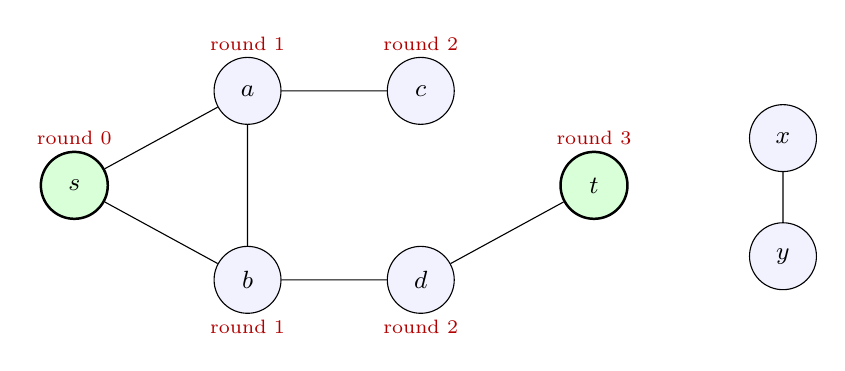
\begin{tikzpicture}[v/.style={circle,draw,minimum size=8.5mm,inner sep=0pt,font=\small,fill=blue!5},
  tt/.style={v,fill=green!15,line width=0.9pt}]
  \node[tt] (s) at (0,0) {$s$};
  \node[v] (a) at (2.2,1.2) {$a$};
  \node[v] (b) at (2.2,-1.2) {$b$};
  \node[v] (c) at (4.4,1.2) {$c$};
  \node[v] (d) at (4.4,-1.2) {$d$};
  \node[tt] (t) at (6.6,0) {$t$};
  \node[v] (x) at (9,0.6) {$x$};
  \node[v] (y) at (9,-0.9) {$y$};
  \draw (s)--(a) (s)--(b) (a)--(c) (b)--(d) (d)--(t) (a)--(b) (x)--(y);
  \foreach \n/\r/\dy in {s/0/6,a/1/6,b/1/-6,c/2/6,d/2/-6,t/3/6}{\node[font=\scriptsize,text=red!70!black] at ([yshift=\dy mm]\n) {round \r};}
\end{tikzpicture}

{\footnotesize Marking rounds starting from $s$: $t$ is marked in round 3, so the machine accepts. $x$ and $y$ are never marked (another component).}
\end{center}

\textbf{Correctness.} By induction, after round $i$ the marked vertices are exactly those at distance $\le i$ from $s$. So when no new vertex is marked, the marked vertices are exactly those reachable from $s$, and $t$ is marked iff an $s$--$t$ path exists.

\textbf{Halting.} Each round except the last marks at least one new vertex, so there are at most $|V|$ rounds, and each round is a finite scan of the edge list. Hence $M$ always halts (in time polynomial in the input length).
\end{soln}

\begin{question}{18}
Describe a Turing machine that, given an encoding of an undirected graph $G=(V,E)$, decides whether the graph contains a cycle. You may assume the input lists the vertices first, followed by the edges. Explain why the machine halts on every valid input.
\end{question}
\begin{soln}
\textbf{Key fact.} An edge $\{u,v\}$ lies on a cycle $\iff$ $u$ and $v$ are still connected after deleting that edge. (The rest of the cycle is a second route from $u$ to $v$.)

Deleting the edge is what prevents the false ``cycle'' $u\to v\to u$ that walks along the same edge and back.

\begin{center}
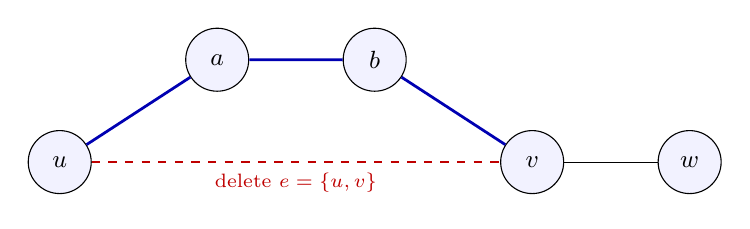
\begin{tikzpicture}[v/.style={circle,draw,minimum size=8mm,inner sep=0pt,font=\small,fill=blue!5}]
  \node[v] (u) at (0,0) {$u$};
  \node[v] (a) at (2,1.3) {$a$};
  \node[v] (b) at (4,1.3) {$b$};
  \node[v] (v) at (6,0) {$v$};
  \node[v] (w) at (8,0) {$w$};
  \draw[line width=1pt,blue!70!black] (u)--(a)--(b)--(v);
  \draw[line width=1pt,red!75!black,dashed] (u)--node[below,font=\scriptsize]{delete $e=\{u,v\}$} (v);
  \draw (v)--(w);
\end{tikzpicture}

{\footnotesize After deleting $e$, $u$ and $v$ are still connected (blue path), so $e$ is on the cycle $u,a,b,v,u$. For $e'=\{v,w\}$, deleting it disconnects $v$ from $w$, so $e'$ is on no cycle.}
\end{center}

$C=$ ``On input $\enc{G}$:
\begin{enumerate}
\item Check the encoding; if invalid, \emph{reject}.
\item For each edge $e=\{u,v\}$ in the list:\\
\hspace*{1.5em}run the path decider $M$ of Q17 on $\enc{G-e,\,u,\,v}$; if it accepts, \emph{accept}.
\item \emph{Reject}.''
\end{enumerate}
(If self-loops $\{u,u\}$ or repeated edges are allowed in the encoding, they form cycles: accept them directly in stage 1.)

\textbf{Correctness.} If $G$ has a cycle, then for any edge $e=\{u,v\}$ on it, the rest of the cycle is a $u$--$v$ path in $G-e$, so stage 2 accepts. Conversely, if $G-e$ has a $u$--$v$ path $P$, then $P$ followed by $e$ is a cycle in $G$ (in a simple graph $P$ has length $\ge2$, as $e$ was removed).

\textbf{Halting.} Stage 2 makes $|E|$ calls to $M$, and $M$ always halts (Q17). So $C$ always halts.

\emph{Alternative:} $G$ is acyclic (a forest) $\iff |E|=|V|-c$, where $c$ is the number of connected components; so $G$ has a cycle $\iff |E|>|V|-c$. Counting components with the marking procedure of Q17 gives another decider.
\end{soln}

\begin{question}{19}
Consider the problem of determining whether a given DFA accepts at least one string. Describe an algorithm for solving this problem and explain why it always terminates.
\end{question}
\begin{soln}
The language is $\{\enc{A}\mid A \text{ is a DFA and } L(A)\neq\emptyset\}$.

\textbf{Key fact.} $A$ accepts some string $\iff$ some accept state can be reached from the start state by following transitions (the labels along the path spell an accepted string). So this is just graph reachability on the state diagram.

$T=$ ``On input $\enc{A}$, $A=(Q,\Sigma,\delta,q_0,F)$:
\begin{enumerate}
\item Mark $q_0$.
\item Repeat until no new state is marked: mark every state $\delta(p,a)$ with $p$ marked and $a\in\Sigma$.
\item If some state of $F$ is marked, \emph{accept}; otherwise \emph{reject}.''
\end{enumerate}
(This is Sipser's $E_{\mathrm{DFA}}$ decider, Thm 4.4, with accept and reject swapped.)

\textbf{Termination.} Each round except the last marks a new state, and there are only $|Q|$ states, so there are at most $|Q|$ rounds, each finite. Note that we never try strings one by one; $L(A)$ may be infinite, but the state graph is finite.
\end{soln}

\begin{question}{20}
For the following language, determine whether it is decidable or undecidable:
$T=\{\enc{G,H}\mid G,H \text{ are CFGs where } L(G)\cap L(H)\neq\emptyset\}$.
\end{question}
\begin{soln}
\textbf{$T$ is undecidable} (though it is Turing-recognizable).

\textbf{Why the obvious approach fails.} CFLs are \emph{not} closed under intersection, so we cannot build a CFG for $L(G)\cap L(H)$ and test emptiness (as we did for DFAs).

\textbf{Proof: reduce PCP to $T$.} Recall (Sipser Thm 5.15) that PCP is undecidable: given dominoes $\bigl[\tfrac{t_1}{b_1}\bigr],\dots,\bigl[\tfrac{t_k}{b_k}\bigr]$, is there a sequence $i_1,\dots,i_m$ ($m\ge1$) with $t_{i_1}\cdots t_{i_m}=b_{i_1}\cdots b_{i_m}$?

Given an instance $P$, take new symbols $a_1,\dots,a_k$ (one ``index'' symbol per domino) and build two grammars:
\[
G_{\mathrm{top}}:\ S\to t_i\,S\,a_i \;\mid\; t_i\,a_i,
\qquad\qquad
G_{\mathrm{bot}}:\ S\to b_i\,S\,a_i \;\mid\; b_i\,a_i
\qquad(i=1,\dots,k).
\]
Then
\[
L(G_{\mathrm{top}})=\{\,t_{i_1}\cdots t_{i_m}\,a_{i_m}\cdots a_{i_1}\,\},\qquad
L(G_{\mathrm{bot}})=\{\,b_{i_1}\cdots b_{i_m}\,a_{i_m}\cdots a_{i_1}\,\}.
\]
The suffix $a_{i_m}\cdots a_{i_1}$ records which dominoes were used.

\textbf{Claim:} $P$ has a match $\iff L(G_{\mathrm{top}})\cap L(G_{\mathrm{bot}})\neq\emptyset$.
\begin{itemize}
\item[($\Rightarrow$)] If $i_1,\dots,i_m$ is a match, then the string $t_{i_1}\cdots t_{i_m}a_{i_m}\cdots a_{i_1}=b_{i_1}\cdots b_{i_m}a_{i_m}\cdots a_{i_1}$ is in both languages.
\item[($\Leftarrow$)] Suppose a string $z$ is in both. The $a$'s do not occur in any $t_i,b_i$, so the index suffix of $z$ is the same in both derivations. Hence both used the same sequence $i_1,\dots,i_m$, and removing the suffix gives $t_{i_1}\cdots t_{i_m}=b_{i_1}\cdots b_{i_m}$: a match.
\end{itemize}
The map $P\mapsto\enc{G_{\mathrm{top}},G_{\mathrm{bot}}}$ is computable, so $\mathrm{PCP}\redm T$. If $T$ were decidable, PCP would be decidable. Contradiction. Hence $T$ is undecidable.

\textbf{$T$ is recognizable:} try strings $z=\eps,0,1,00,\ldots$ in order, and use the $A_{\mathrm{CFG}}$ decider (Thm 4.7) to test $z\in L(G)$ and $z\in L(H)$. Accept if both hold. So $\comp T$ (``the intersection is empty'') is not even recognizable (otherwise $T$ would be decidable by Thm 4.22).
\end{soln}
